\documentclass{article}
\usepackage{graphicx}
\usepackage{amsmath}
\begin{document}
\title{CS 124 Problem Set 5}
\author{Author: 30943147. I collaborated with 50996336.}
\maketitle

\section*{Problem 1}
\subsection*{a}
We are hashing $k \geq c_1 \sqrt{n}$ people into $n$ bins. The probability that no two have the same hash is equal to
$$\prod\limits_{i=0}^k (1-\frac{i}{n}) \leq \prod\limits_{i=0}^k (e^{-i}) = e^{-\sum\limits_{i=0}^k \frac{i}{n}} = e^{\frac{k(k+1)}{2n}} \leq e^{\frac{c_1 \sqrt{n} (c_1 \sqrt{n} + 1)}{2n}} \leq e^{\frac{-c_1^2}{2}}$$
The last step above follows from $n \geq 1$. Choosing $c_1 \geq \sqrt{2}$ then gives the probability that no two have the same hash as $\leq e^{-1}$.

\subsection*{b}
Let P be the probability that no two people share a birthday. Using the identity $1-x \geq e^{-x-x^2}$ (which is valid since $x \leq \frac{c_2 \sqrt{n}}{n} \leq \frac{1}{2}$ since we are working with "sufficiently large $n$"), we get
$$P \geq \prod_{i=0}^k e^{\frac{-i}{n} - \frac{i^2}{n^2}} = e^{-\frac{k (k+1)}{2n} - \frac{k (k+1) (2k + 1)}{6 n^2}}
 \geq  e^{-\frac{c_2 \sqrt{n} (c_2 \sqrt{n} +1)}{2n} - \frac{c_2 \sqrt{n} (c_2 \sqrt{n}+1) (2c_2 \sqrt{n} + 1)}{6 n^2}}$$
We want to choose $c_2$ such that 
$$e^{-\frac{c_2 \sqrt{n} (c_2 \sqrt{n} +1)}{2n} - \frac{c_2 \sqrt{n} (c_2 \sqrt{n}+1) (2c_2 \sqrt{n} + 1)}{6 n^2}} \geq \frac{1}{2}$$
We take the log and simplify. 
$$\frac{c_2 \sqrt{n} (c_2 \sqrt{n} +1)}{n} + \frac{c_2 \sqrt{n} (c_2 \sqrt{n}+1) (2c_2 \sqrt{n} + 1)}{3 n^2} \leq 2 \ln (2)$$
Since $n$ is "sufficiently large", all terms with a negative power of $n$ are negligable compared to the constant terms, and we reduce this expression to
$$c_2^2 \leq 2 \ln 2$$
$$c_2 \leq \sqrt{2 \ln 2}$$

\section*{Problem 2}
\subsection*{a}
We are hashing $n$ elements into $k$ hashtables, each of size $\frac{m}{k}$. Each slot in the table has $b$ bits. Therefore, hashing $\geq 2^b$ elements into that slot will produce overflow.  First, we find the probability that an arbitrarily chosen slot doesn't overflow (all slots are identical for this purpose). Call that probability $X$. $X$ is equal to the probability that the slot has $< 2^b$ elements. The probability that the slot has $i$ elements is equal to 
$$(\frac{k}{m})^i (\frac{m-k}{m})^{n-i} {n \choose i}$$
Therefore, $X_i$ is equal to 
$$X = \sum\limits_{i=0}^{2^{b-1}} (\frac{k}{m})^i (\frac{m-k}{m})^{n-i} {n \choose i}$$
The probability that our arbitrarily chosen slot overflows is then equal to 
$$P = 1-X = 1-(\sum\limits_{i=0}^{2^{b-1}} (\frac{k}{m})^i (\frac{m-k}{m})^{n-i} {n \choose i})$$
\subsection*{b}

\section*{Problem 3}
\subsection*{a}
Generally, we have the probability of matching using a single sketch as
$$p(r) = \sum\limits_k^n {n \choose k} r^k (1-r)^{n-k}$$
So, for our initial hashing, we have
$$p(r) =  \sum\limits_k^{84} {84 \choose k} r^k (1-r)^{84-k}$$
For the rehashing, we have $k=2$, $n = 6$, and $r' = r^{14}$, which is the probability that all $14$ values input into a given hash match. For now, we are assuming no collisions. This is a reasonable assumption because we are hashing $14$ values into a hashtable of size $2^{64}$, so the probability of collisions will be tiny. Regardless, a small number of false positives is not a problem--it will only result in a few websites being marked as duplicate when they shouldn't be. The probability $p'(r)$ of a match using this rehashing is
$$p'(r) = \sum\limits_{k=2}^6 {6 \choose k} r^{14k} (1-r^{14})^{6-k}$$
Graphing $p'(r)$ with Mathematica gives the following graph, where the verticle axis is $p'(r)$ and the horizontal axis is $r$. \\
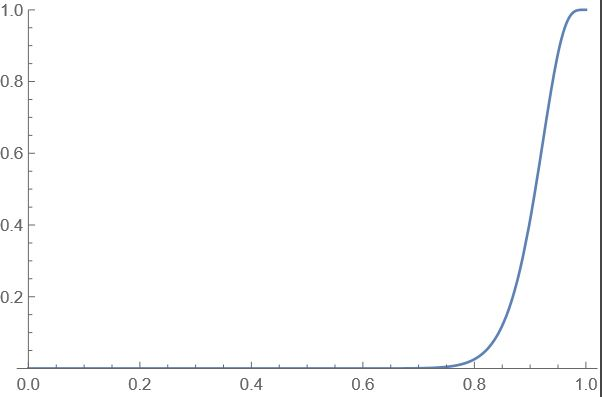
\includegraphics[scale=0.7]{pset5_3_graph.jpg}

Evaluating $p'(r)$ for select values of $r$ gives the following results: \\
\begin{center}
\begin{tabular}{ | c | c | }
\hline
$r$ & $p'(r)$ \\
\hline\hline
0.70 & 0.00068 \\
\hline
0.75 & 0.0045\\
\hline
0.80 & 0.026\\
\hline
0.85 & 0.12\\
\hline
0.90 & 0.42\\
\hline
0.95 & 0.88\\
\hline
0.98 & 0.996 \\
\hline
0.99 & 0.9998 \\ 
\hline

\end{tabular}
\end{center}
We can see that documents with resemblance $\leq$ 0.75 have only a tiny chance of being marked as duplicate, and documents with resemblance $\geq$ 0.98 have onlly a tiny chance of being marked as not duplicate.  
\subsection*{b}
Now we turn our attention to the possibility of collisions. We must modify our equation
$$p'(r) = \sum\limits_{k=2}^6 {6 \choose k} r^{14k} (1-r^{14})^{6-k}$$
by replacing $r^14$ with $r^14 + (1-r^{14}) \frac{1}{H}$, where $H$ is the size of our hashtable. $r^14$ is the probability that the group matches, and $(1-r^{14}) \frac{1}{H}$ is the probability that the group does not match but they happen to hash the same regardless. Making the correction for the 64-bit hash, ie $H = 2^{64}$, results in negligible changes
$$p_{64}(r) = \sum\limits_{k=2}^6 {6 \choose k} (r^{14} + (1-r^{14}) \frac{1}{2^{64}})^k (1-r^{14})^{6-k}$$
Plotting $p_{64}(r)$ gives\\
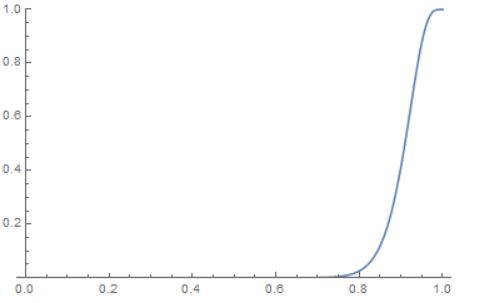
\includegraphics[scale=0.8]{p64.jpg}

Evaluating $p_{64}(r)$ at select values gives the exact same table of values (at least to the level of precision we have decided to use)
\begin{center}
\begin{tabular}{ | c | c | }
\hline
$r$ & $p_{64}(r)$ \\
\hline\hline
0.70 & 0.00068 \\
\hline
0.75 & 0.0045\\
\hline
0.80 & 0.026\\
\hline
0.85 & 0.12\\
\hline
0.90 & 0.42\\
\hline
0.95 & 0.88\\
\hline
0.98 & 0.996 \\
\hline
0.99 & 0.9998 \\ 
\hline

\end{tabular}
\end{center}
This confirms our assumption in part a that the possibility of a collision on 64-bit hash values is negligible. 

Now consider 16-bit hashtables
$$p_{16}(r) = \sum\limits_{k=2}^6 {6 \choose k} (r^{14} + (1-r^{14}) \frac{1}{2^{16}})^k (1-r^{14})^{6-k}$$
Plotting $p_{16}$ gives\\
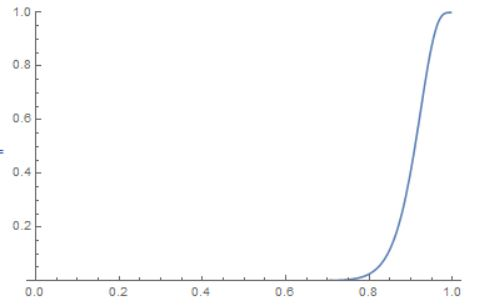
\includegraphics[scale=0.8]{p16.jpg}

\begin{center}
\begin{tabular}{ | c | c | }
\hline
$r$ & $p_{16}(r)$ \\
\hline\hline
0.70 & 0.00068 \\
\hline
0.75 & 0.0045\\
\hline
0.80 & 0.026\\
\hline
0.85 & 0.12\\
\hline
0.90 & 0.42\\
\hline
0.95 & 0.88\\
\hline
0.98 & 0.996 \\
\hline
0.99 & 0.9998 \\ 
\hline

\end{tabular}
\end{center}
The differences do not show up in our 2-significant figure tables, but they are visible when looking at the longer forms of the decimals that Mathematica spits out. 

Now consider 8-bit hashtables
$$p_{8}(r) = \sum\limits_{k=2}^6 {6 \choose k} (r^{14} + (1-r^{14}) \frac{1}{2^{8}})^k (1-r^{14})^{6-k}$$
The plot now looks slightly different from the 64-bit case even to the naked eye
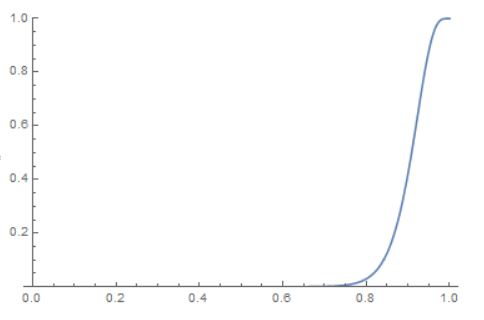
\includegraphics[scale=0.8]{p8.jpg}

\begin{center}
\begin{tabular}{ | c | c | }
\hline
$r$ & $p_{16}(r)$ \\
\hline\hline
0.70 & 0.0017 \\
\hline
0.75 & 0.0067\\
\hline
0.80 & 0.030\\
\hline
0.85 & 0.13\\
\hline
0.90 & 0.43\\
\hline
0.95 & 0.89\\
\hline
0.98 & 1.00 \\
\hline
0.99 & 1.00 \\ 
\hline

\end{tabular}
\end{center}
8-bit hashing produces noticeable differences compared to the 64-bit case, especially for the lower values of $r$. We probably do not want to mark a pair of documents with only 75 or 80 percent resemblance as duplicates, and the 8-bit hash makes it much more likely that we will do so than the 16 or 64-bit hash. 

\section*{Problem 4}

\section*{Problem 5}
The code used in problem 5 is submitted as q5.java
\subsection*{a}
We show that $n=636127$ is composite using Fermat's little theorem. We adapt our code from problem 6 (which I did first) to calculate
$$2^{n-1} \mod n = 2^{318063} \mod 636127 = 469435 \neq 1$$
$n=636127$ fails Fermat's little theorem for $a=2$, and therefore cannot be prime.  
\subsection*{b}
We show that $n=294409$ is composite using the Rabin-Miller primality test with $a=2$. First, we decompose $n = 2^t u$ for $t=3$ and $u=36801$. Now, we use our power mod code in q5.java to calculate the following values (which I then checked with Mathematica's power mod function). 

\begin{center}
\begin{tabular}{ | c | c |}
\hline
$ 2^u \mod n$ & $512$ \\
\hline
$ 2^{2u} \mod n$ & $262144$ \\
\hline
$ 2^{4u} \mod n$ & $1$ \\
\hline
$ 2 ^ {8u} \mod n = 2^{n-1} \mod n$ & $1$ \\
\hline
\end{tabular}
\end{center}
We have found that $2^{2u}$ is a non-trivial square root of $2^{4u}$. Therefore, by the Rabin-Miller primality test, $n$ is composite. 


\end{document}